\chapter{Hardware Layer}
\label{chap:hardware}
\begin{comment}

\begin{figure*}[t]
    \centering
      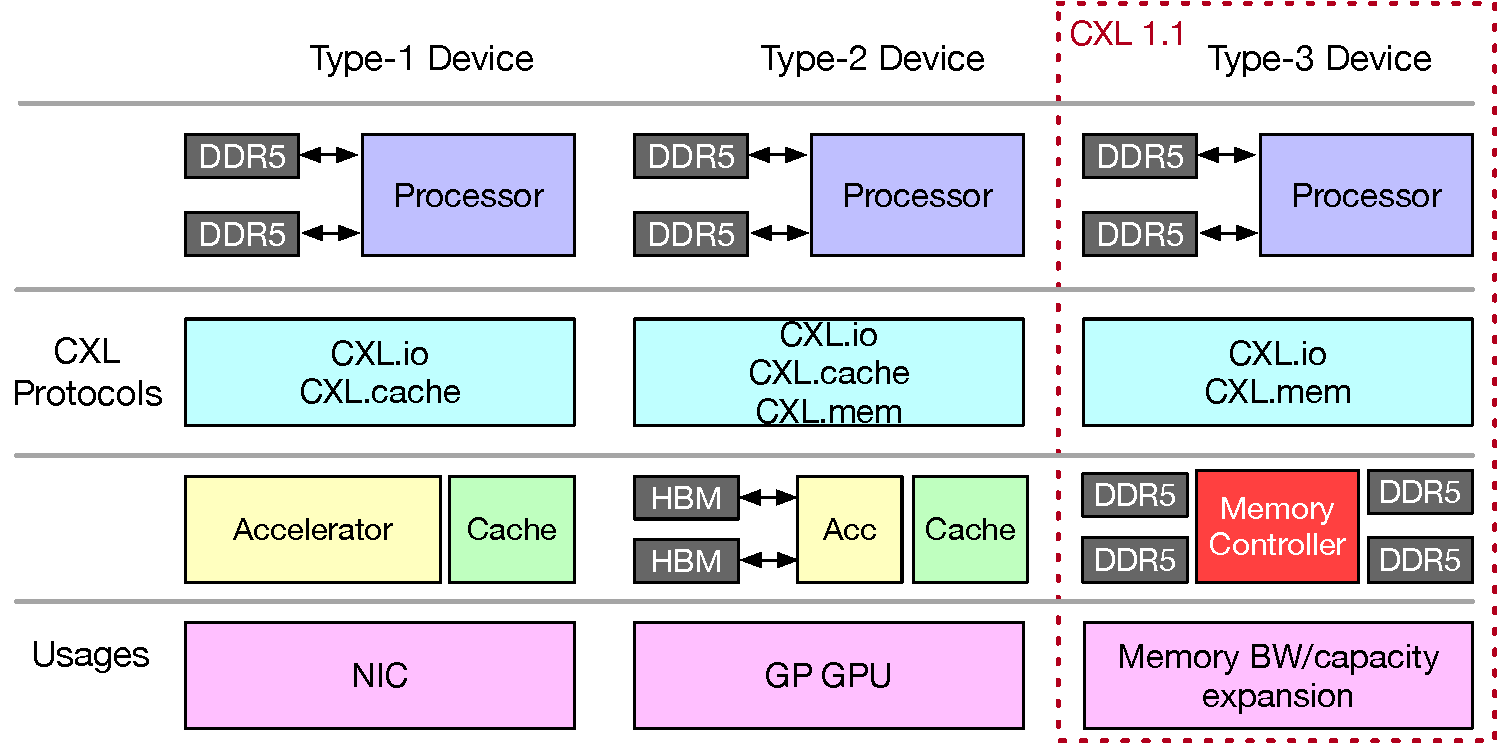
\includegraphics[width=\textwidth]{cxl}
      \caption{\textbf{CXL Overview}} 
    \label{fig:cxl} \vspace{-1.0em}
    \end{figure*}

\begin{figure}[t]
    \centering
      \includegraphics[width=0.9\columnwidth]{cxl_performance}\vspace{-1.0em}
      \caption{\textbf{CXL Performance for Read-only Workload.} CXL denotes accessing memory through Compute Express Link, while DRAM refers to traditional memory access. The '-r' suffix indicates remote socket access.} \vspace{-2.0em}
    \label{fig:cxlperformance}
    \end{figure}
    
\end{comment}
While network-based resource disaggregation has gained attention due to advancements in network bandwidth (\S\ref{sec:os}), the inherent latency, limited by the speed of light, still imposes significant overheads. This section explores the potential of next-generation interconnects and their impact on resource disaggregation.

\section{Next-generation Interconnects}

Recent advancements in hardware have led to the development of new-generation interconnects by major hardware vendors, such as NVLink~\cite{nvlink} from Nvidia and Compute Express Link (CXL)~\cite{cxl} from Intel. CXL, in particular, has been introduced as a promising solution to expand memory capacity and bandwidth by attaching external memory devices to PCIe slots, offering a dynamic and heterogeneous computing environment.

\paragraphb{Compute Express Link (CXL)}
As depicted in Figure~\ref{fig:cxl}, CXL encompasses three key protocols: CXL.mem, CXL.cache, and CXL.io. CXL.io serves as the PCIe physical layer. CXL.mem enables processors to access memory over PCIe, while CXL.cache facilitates coherent memory access between processors and accelerators. These protocols allow for the construction of various CXL device types. The initial CXL 1.1 version serves as a memory expander for a single server. Subsequent versions, like CXL 2.0, extend this capability to multiple servers, incorporating CXL switches that coordinate access from different servers and enable various compute nodes to share a large memory pool. The forthcoming CXL 3.0 aims to scale up further, with cache coherency managed by hardware.

Despite extensive research on CXL~\cite{cxl_azure,cxlcentric,demystify}, practical, commercial CXL hardware implementations remain in development, posing challenges in fully understanding performance and system support design for such hardware. Most studies have relied on simulations or FPGA-based CXL hardware~\cite{demystify,intelfpga}, lacking empirical evaluations on ASIC-based CXL hardware. Moreover, existing research often focuses on single aspects of CXL, like capacity or bandwidth, using synthetic benchmarks and neglecting a comprehensive evaluation that includes cost considerations. To gauge the performance of real CXL hardware and assess its suitability for resource disaggregation, we evaluated the latest hardware available: Intel's $\text{4}^{th}$ generation scalable processor (Sapphire Rapids) and Asteralabs's CXL 1.1 memory expander (Type-3 device). Using Intel Memory Latency Checker (MLC)\cite{mlc}, we measured the latency of reading data from the CXL device and local memory equipped with the same amount of DDR5 channels for local and cross-socket access. Figure\ref{fig:cxlperformance} reveals that the latest CXL hardware exhibits a latency of more than $2.5\times$ higher than local memory. However, this gap narrows for cross-socket access, suggesting CXL as another memory tier. This raises questions about whether and how this information should be exposed to applications. Previous research~\cite{tpp} has investigated promoting hot pages from slower-tiered memory at the kernel level to enhance performance while maintaining application transparency.

This study represents the first available evaluation of real CXL 1.1 ASICs. The performance of CXL 2.0 and 3.0 remains to be explored in future work.

\subsection{Introduction}
\subsection{Background and Methodology}
\subsection{CXL 1.1 Performance characteristics}
\subsection{Memory Capacity-bound Applications}

\subsection{Memory Bandwidth-bound Applications}

\subsection{Cost Implications}

\subsection{Discussion and Conclusion}

\section{Introduction}

In an era marked by the rise of memory-intensive applications, such as machine learning tasks and High-Performance Computing (HPC), there is an urgent need to expand memory capacity and bandwidth. For example, a machine learning application with a 175 billion parameter model requires 700 GB of memory just to hold its parameters, not including the additional memory needed for intermediate results and other data. As a result, the memory demands of modern applications can easily exceed the capacity of a single machine due to physical constraints, such as the limited availability of DDR DIMM slots and thermal challenges, as well as the high cost of employing high-density DIMMs.

To address these demands, Compute Express Link (CXL) has been introduced as a groundbreaking interconnect technology. CXL promises to significantly expand memory capacity and bandwidth by enabling the attachment of external memory devices (e.g., DRAM, Flash, or persistent memory) to PCIe slots. Unlike its predecessors, CXL fosters a more dynamic and heterogeneous computing environment, leading to various design trade-offs for performance and cost efficiency. Debuting commercially with version 1.1, CXL allows direct attachment of external memory devices to the host machine, creating a unified and coherent memory address space. In this configuration, CXL is primarily used as a means of memory expansion. For instance, AsteraLabs' A1000 CXL memory expansion card supports up to four DDR5 RDIMMs, providing up to 2 TB of additional memory for a single server.

Although substantial research on CXL memory has been conducted, there remains a significant gap in applying these studies to guide the practical integration of CXL. Specifically, we observe the following issues:

Much of the current literature has focused on evaluating CXL hardware through simulations or using FPGA-based setups. While some studies have begun to assess the raw performance of ASIC-based CXL hardware, there is still a lack of understanding of how different system configurations impact the performance of data center applications using CXL memory. Additionally, the specific applications that could significantly benefit from CXL memory expansion have not yet been fully identified.
While existing studies have explored the cost implications of employing CXL technology, such as memory pooling cost models, a critical gap remains in understanding the cost-effectiveness of migrating specific applications or services to memory expansions facilitated by CXL.
Due to the limited availability of CXL ASIC hardware, the research community faces a notable scarcity of open-source empirical data. This limitation hinders efforts to fully comprehend the performance capabilities of such hardware or to develop performance models based on empirical evidence.
Our study aims to address these gaps by conducting detailed evaluations of CXL 1.1 for memory-intensive applications, leading to several key observations: Contrary to the common perception that CXL memory, due to its higher latency, should be considered a separate, slower tier of memory, we find that shifting some workloads to CXL memory can significantly enhance performance, even if local memory's capacity and bandwidth are underutilized. This improvement occurs because using CXL memory can reduce overall memory access latency by alleviating bandwidth contention on DDR channels, thereby improving application performance. From our analysis of application performance, we have developed an abstract cost model that predicts substantial cost savings in practical deployments.

In summary, the major contributions of this paper are:

Empirical Evaluation of ASIC CXL Hardware: Our study provides a comprehensive examination of the performance of ASIC-based CXL hardware and system configurations in data center applications, offering insights on optimizing CXL memory utilization.
Cost-Benefit Analysis: We conduct a thorough cost-benefit analysis and develop an abstract cost model to evaluate how CXL memory could significantly reduce the Total Cost of Ownership (TCO) for real-world applications.
Open-source Data on CXL ASIC Performance: We make all data and testing configurations publicly available at \url{https://github.com/bytedance/eurosys24-artifacts}.
The paper is organized as follows: \S\ref{sec
} introduces the basic concepts of CXL and the setup for our evaluations. \S\ref{sec
} presents the basic performance characteristics of CXL memory expansion. \S\ref{sec
} and \S\ref{sec
} discuss findings and recommendations for using CXL to expand memory capacity and bandwidth in data center workloads. \S\ref{sec
} provides a detailed analysis of the potential cost benefits offered by CXL. \S\ref{sec
} explores how our insights apply to future generations of CXL. \S\ref{sec
} reviews related work, and \S\ref{sec
} concludes the paper.







\section{Background and Methodology} \label{sec
}

This section provides an overview of CXL technology, followed by details on our experimental setup and methodologies.

\subsection{Compute Express Link (CXL) Overview}

Compute Express Link (CXL) is a standardized interconnect technology that facilitates communication between processors and various devices, such as accelerators, memory expansion units, and smart I/O devices. CXL is built on the physical layer of PCI Express (PCIe) 5.0, supporting x16, x8, and x4 link widths with data rates of 32.0 GT/s and 64.0 GT/s. The CXL transaction layer is implemented through three protocols: CXL.io, CXL.cache, and CXL.mem. The CXL.io protocol is based on PCIe 5.0 and handles device discovery, configuration, initialization, I/O virtualization, and direct memory access (DMA). CXL.cache allows CXL devices to access the host processor's memory, while CXL.mem enables the host to access memory attached to devices using load/store commands.

CXL devices are categorized into three types, each tailored for specific use cases:

Type-1 devices, such as SmartNICs, utilize CXL.io and CXL.cache for DDR memory communication.
Type-2 devices, including GPUs, ASICs, and FPGAs, use CXL.io, CXL.cache, and CXL.mem to share memory with the processor, enhancing workloads within the same cache domain.
Type-3 devices leverage CXL.io and CXL.mem for memory expansion and pooling, increasing DRAM capacity, enhancing memory bandwidth, and enabling the addition of persistent memory without sacrificing DRAM slots. Type-3 devices complement DRAM with CXL-enabled solutions, benefiting high-speed, low-latency storage.
The commercially available version of CXL is 1.1, where a CXL 1.1 device functions as a single logical device accessible by one host at a time. Future generations of CXL, such as CXL 2.0, are expected to support the partitioning of devices into multiple logical units, allowing up to 16 different hosts to access different portions of memory. This paper focuses on commercially available CXL 1.1 Type-3 devices, specifically addressing single-host memory expansion.

\subsection{Hardware Support for CXL} \label{ssec
}

Recent advancements have introduced CXL 1.1 support in Intel Sapphire Rapids processors (SPR) and AMD Zen 4 EPYC "Genoa" and "Bergamo" processors. While commercial CXL memory modules are provided by vendors such as AsteraLabs, Montage, Micron, and Samsung, CXL memory expanders are predominantly in prototype stages, with limited availability, making access difficult for university labs. Consequently, research into CXL memory has primarily relied on NUMA-based emulation and FPGA implementations, each with inherent limitations.

\paragraphb{NUMA-based Emulation} Given the cache-coherent nature and comparable transfer speeds of CXL and UPI/xGMI interconnects, NUMA-based emulation is widely adopted to enable fast application performance analysis and software prototyping, with CXL memory exposed as a remote NUMA node. However, NUMA-based emulation fails to accurately capture the performance characteristics of CXL memory due to differences between CXL and UPI/xGMI interconnects, as shown in previous research.

\paragraphb{FPGA-based Implementation} Intel and other hardware vendors use FPGA hardware to implement CXL protocols, bypassing the performance inconsistencies of NUMA-based emulation. However, FPGA-based CXL memory falls short in fully utilizing memory chip performance due to its lower operating frequency compared to ASICs. FPGAs prioritize flexibility over performance and are suitable for early-stage CXL memory validation but not for production deployment. Recent evaluations have uncovered performance issues in FPGA implementations, including reduced memory bandwidth during concurrent thread execution, which hampers rigorous evaluations for memory capacity- and bandwidth-bound applications—key use cases for CXL memory expanders.

To the best of our knowledge, we are among the first to uncover the performance characteristics of actual ASIC prototypes designed for CXL memory expansion. The ASIC CXL memory controller we employed is the A1000 developed by AsteraLabs, which implements the CXL interface at speeds of up to 32 GT/s per lane, supporting up to 16 lanes in total. This controller can accommodate up to four DDR5-5600 RDIMM slots, providing a total memory capacity of 2TB.

\subsection{Software Support for CXL} \label{ssec
}

While hardware vendors are actively advancing CXL production, there is a notable deficiency in software and OS kernel support for CXL memory, prompting the utilization of specific software enhancements. We summarize the most recent patches in the Linux Kernel that add CXL-aware support, namely: (1) the interleaving policy support (unofficial) and (2) the hot page selection support (official since Linux Kernel v6.1).

\paragraphb{N
Interleave Policy for Tiered Memory Nodes} Traditional memory interleave policies distribute data evenly across memory banks, often using a 1:1 ratio. However, the advent of tiered memory systems, which feature CPU-less memory nodes with diverse performance traits, demands more nuanced strategies for optimizing memory bandwidth, especially for bandwidth-heavy applications. The interleave patch introduces an innovative N
interleave policy to address this, allowing for an allocation scheme where N pages are directed to high-performance (top-tier) nodes and M pages to lower-tier nodes. For example, using a 4:1 ratio directs 80% of traffic to top-tier nodes and 20% to low-tier nodes, adjustable through the vm.numa_tier_interleave parameter. While the patch showcases compelling evaluation results, it's crucial to note that optimal memory distribution depends on specific hardware and application characteristics. Given the higher latency of CXL memory, performance-sensitive applications should undergo thorough profiling and benchmarking to maximize the advantages of interleaving and mitigate potential performance trade-offs.

\paragraphb{NUMA Balancing and Hot Page Selection} The memory subsystem, now termed a memory tiering system, accommodates various memory types like PMEM and CXL Memory, each with differing performance characteristics. To optimize system performance, "hot pages" (frequently accessed) should reside in faster memory tiers like DRAM, while "cold pages" (less frequently accessed) should be in slower tiers like CXL memory. Recent Linux Kernel patches address this:

The \textit{NUMA-balancing} patch uses a latency-aware page migration strategy, focusing on promoting recently accessed pages (MRU). It scans NUMA balancing page tables and hints page faults. However, it may not accurately identify high-demand pages due to extended scanning intervals, potentially causing latency issues for some workloads.

The \textit{Hot Page Selection} patch introduces a Page Promotion Rate Limit (RPRL) mechanism to control the rate of page promotions and demotions. While this extends promotion/demotion times, it improves workload latency. The hot page threshold is dynamically adjusted to align with the promotion rate limit.

Additionally, research prototypes like TPP share a similar concept with optimizations and are being considered for integration into the Linux Kernel. However, we faced challenges with TPP when running memory-bandwidth-intensive applications, resulting in unexplained performance degradation. Hence, we rely on the well-tested kernel patches integrated into Linux Kernel since version 6.1.

\subsection{Experimental Platform Description}

The evaluation testbed consists of three servers. Two of these servers are designated as CXL experiment servers. Each of these servers is equipped with dual Intel Xeon 4th Generation CPUs (Sapphire Rapids, or SPR), 1 TB of 4800 MHz DDR5 memory, two 1.92 TB SSDs, and a pair of A1000 CXL Gen5 x16 ASIC memory expander modules from AsteraLabs, each with 256 GB of 4800 MHz memory (resulting in a total of 512 GB memory per server). Both A1000 memory modules are attached to socket 0. The third server serves as the baseline and is configured identically to the CXL experiment servers, except for the absence of the CXL memory expanders. It is designated for initiating client requests and running workloads that strictly utilize the main memory during the application assessments. All servers are interconnected via 100 Gbps Ethernet links.


\section{CXL 1.1 Performance Characteristics} \label{sec
}

In this section, we assess the performance of the CXL memory expander and compare it directly with main memory, which we designate as \textbf{MMEM} for clarity against CXL memory. We analyze workload patterns and evaluate performance differences between local and remote socket scenarios.

\subsection{Experimental Configuration} \label{ssec
} For each dual-channel A1000 ASIC CXL memory expander, we connect two DDR5-4800 memory channels, achieving a total capacity of 256 GB. To provide a fair comparison between MMEM and CXL-attached DDR5 memory, we utilize the Sub-NUMA Clustering (SNC) feature to ensure the number of memory channels is the same in both settings.

\paragraphb{Sub-NUMA Clustering(SNC)} Sub-NUMA Clustering (SNC) serves as an enhancement over the traditional NUMA architecture. It decomposes a single NUMA node into multiple smaller semi-independent sub-nodes (domains). Each sub-NUMA node possesses its own dedicated local memory, L3 caches, and CPU cores. In our experimental setup, we partition each CPU into four sub-NUMA nodes. Each sub-NUMA node is equipped with two DDR5 memory channels connected to two 64 GB DDR5-4800 DIMMs. Enabling SNC requires setting the IMC (Integrated Memory Controllers) to 1-way interleaving. According to the specifications, a single DDR5-4800 channel has a theoretical peak bandwidth of 38.4 GB/s. Therefore, each sub-NUMA node has a combined memory bandwidth of up to 76.8 GB/s.

\paragraphb{Intel Memory Latency Checker (MLC)} We leverage Intel's Memory Latency Checker (MLC) to examine loaded latency for various read-write workloads, adopting a 64-byte access size the same as prior work. We deploy 16 MLC threads, and it’s important to note that while the thread count is a configurable parameter in MLC, it doesn’t directly dictate memory request concurrency. MLC assigns separate memory segments for each thread to access simultaneously. Specifically, when evaluating loaded latency, MLC incrementally increases the operation rate of each thread. Our findings indicate that employing 16 threads with MLC precisely measures both the idle and loaded latency and the point at which bandwidth becomes saturated. MLC accommodates a broad spectrum of workloads, including those with varied read-write mixes and non-temporal writes.

Our study is focused on addressing the following research questions:

\begin{icompact} \item How is the performance of the CXL-attached memory compared to that of local-socket/remote-socket main memory? \item What is the performance impact of the CXL memory under different read-write ratios and access patterns (random vs. sequential)? \item How do main memory and CXL memory behave under high memory load conditions? \end{icompact}

\subsection{Basic Latency and Bandwidth Characteristics} \label{ssec
} This section outlines our findings on memory access latency and bandwidth for different memory configurations: local-socket main memory (MMEM), remote-socket main memory (MMEM-r), CXL memory (CXL), and remote-socket CXL memory (CXL-r). We observe that MMEM achieves a peak bandwidth of roughly 67 GB/s, reaching 87% of its theoretical maximum. However, as write operations increase, bandwidth dips, with write-only tasks dropping to 54.6 GB/s. The initial memory latency is about 97 ns, which spikes exponentially as bandwidth nears full capacity, indicating bandwidth contention. Interestingly, latency begins to significantly increase at 75%-83% of bandwidth utilization, surpassing prior estimates of 60% from earlier studies.

When accessing MMEM via a remote socket, latency begins at approximately 130 ns for read-only tasks, contrasting sharply with just 71.77 ns for write-only operations. This reduced latency for write-only workloads results from non-temporal writes, which proceed asynchronously without awaiting confirmation. Despite read-only tasks achieving maximum bandwidth comparable to that of local MMEM, incorporating more write operations significantly diminishes bandwidth, attributed to the additional UPI traffic necessitated by cache coherence protocols. Interestingly, write-only workloads generate minimal UPI traffic but suffer the lowest bandwidth as they utilize only one direction of the UPI's bidirectional capabilities. Moreover, latency escalation occurs earlier in remote socket memory accesses than in local ones, primarily due to queue contention at the memory controller.

The latency curve for CXL memory expansion demonstrates a minimum latency of 250.42 ns. Despite additional PCIe and CXL memory controller overhead on the datapath, accessing CXL follows the same "Bandwidth contention" trend as MMEM. The latency of accessing CXL on the same socket remains relatively stable as bandwidth increases, with a maximum bandwidth of around 56.7 GB/s, achieved when the workload has a 2:1 read-write ratio. The reduction in maximum bandwidth compared to DRAM is attributed to PCIe overhead, such as extra headers. The maximum bandwidth for read-only workloads is smaller due to PCIe bi-directionality, preventing full bandwidth utilization. Accessing CXL from a remote socket incurs an exceptionally high idle latency of 485 ns. Additionally, the maximum memory bandwidth is unexpectedly halved, reaching just 20.4 GB/s for a 2:1 read-write ratio, which is a much more severe performance drop compared to accessing MMEM from the remote NUMA node. Since running a read-only workload towards a CXL Type-3 device on the remote socket does not generate substantial coherence traffic, initial speculation regarding cache coherence is ruled out. Further investigation utilizing the Intel Performance Counter Monitor (PCM) also confirms that UPI utilization is consistently below 30\%. Discussions with Intel suggest this performance bottleneck is likely due to limitations in the Remote Snoop Filter (RSF) on the current CPU platform, anticipated to be addressed in the next-generation processors.

\subsection{Different Read-Write Ratios \& Access Pattern}

We observe that accessing CXL from a remote socket introduces exceptionally high latency and low bandwidth. When accessing CXL from the same socket, latency is 2.4-2.6 times that of local DDR and 1.5-1.92 times that of remote socket DDR. This suggests that running applications directly on CXL may significantly reduce performance. However, when workloads span multiple NUMA nodes within the same socket, accessing CXL locally is comparable to accessing remote NUMA node memory. Additionally, the latency-bandwidth knee-point shifts to the left as the proportion of write operations in the workload increases. Notably, we do not observe any significant performance disparities when running both read-only and write-only workloads utilizing random access patterns instead of sequential access.

\subsection{Key insights} \paragraph{Avoiding Remote Socket CXL Access.} CXL memory expansion is commonly utilized for memory-demanding applications, particularly those limited by memory capacity or bandwidth. In such contexts, accessing memory across sockets is not uncommon. It is important for software developers to recognize the potential decline in performance when CXL memory is accessed from a remote socket and to strategize against cross-socket CXL memory accesses in their applications. Additionally, hardware vendors should perform cooperative testing and validation of their products to ensure compatibility between CXL memory modules and the processors' CXL support. With adequate support for the CXL 1.1 protocol, we expect that the maximum bandwidth attainable when accessing CXL memory across sockets could approximate the bandwidth seen when accessing MMEM across sockets.

\paragraph{Bandwidth Contention} Previous research has highlighted issues related to bandwidth contention. We further examine how memory latency varies with different read-write ratios under bandwidth contention. While latency remains relatively stable at low to moderate bandwidth utilization levels, it increases exponentially as bandwidth approaches higher levels, primarily due to queuing delays in the memory controller. Furthermore, the knee-point in latency shifts to lower memory bandwidth when there is a higher proportion of write operations in the workload. Interestingly, CXL-attached memory has often been characterized by the industry and research community as 'tiered memory,' suggesting that it serves as a slower and less performant memory layer to be considered only when MMEM is fully utilized. However, we argue against this simplistic view of CXL memory. Allocators and kernel-level page placement policies should consider the available bandwidth in MMEM. Even if a substantial portion of memory bandwidth in MMEM remains unused, e.g., 30%, offloading a portion of the workload, e.g., 20%, to CXL memory can lead to overall performance improvements. Our recommendation is to regard CXL memory as a valuable resource for load balancing, even when local DRAM bandwidth is not fully utilized. Subsequent real-world evaluations support these insights.

\paragraph{Comparison with FPGA-based CXL implementations.} Intel recently disclosed latency and bandwidth performance metrics for their FPGA-based CXL prototype. While they provided insights into relative latency and bandwidth efficiency for soft and hard IP implementations, performance under load was not shared. Our measurements indicate that the ASIC CXL solution introduces less than a 2.5x overhead in access latency compared to MMEM, surpassing most of Intel's measurements. However, the FPGA-based solution achieved only 60% of the PCIe bandwidth due to the inefficiency of the memory controller, while the Asteralabs A1000 prototype reached an impressive 73.6% bandwidth efficiency, clearly outperforming Intel's FPGA-based solution.


\section{Memory Capacity-bound Applications} \label{sec
}

One of the most significant advantages of integrating CXL memory into modern computing systems is the opportunity for significantly larger memory capacities. To elucidate the potential benefits, we focus on three particular use cases: (1) key-value stores, a commonly used application in data centers, (2) big data analytical applications, and (3) elastic computing from cloud providers.

\subsection{In-memory key-value stores} \label{ssec
} Redis is an open-source in-memory key-value store and one of the most popular NoSQL databases. Redis employs a user-defined parameter, \texttt{maxmemory}, to limit its memory allocation for storing user data. Like traditional memory allocators (e.g., malloc()), Redis may not return memory to the system after key deletion, particularly if deleted keys were on a memory page with active ones. This necessitates memory provisioning based on peak demand, making memory capacity the major bottleneck for Redis deployments in data centers. Some cloud providers suggest keeping memory usage below 80%, whereas other sources recommend a limit of 75%.

Due to the substantial infrastructure costs for memory-only deployment, Redis Enterprise is the commercial variant extensively supported by leading cloud platforms. It introduces "Auto Tiering" to allow data overflow to SSDs, offering an economically viable option for database expansion beyond the limits of RAM capacity. Given that Redis Enterprise is not accessible on our experiment platform, we employ KeyDB as an alternative. KeyDB extends Redis's capabilities by adding KeyDB Flash, which uses RocksDB for persistent storage. The FLASH feature enables all data to be written to the disk for persistence, with hot data remaining in memory as well as on disk.

\subsubsection{Methodology and Software Configurations}

In our study, we investigate the performance effects of maximizing memory utilization on a KeyDB server. We deploy a single KeyDB instance on a CXL-enabled server configured with seven \textit{server-threads}. Unlike Redis's single-threaded approach, KeyDB enhances performance by operating multiple threads to run the standard Redis event loop, akin to running several Redis instances simultaneously. We disable SNC and Transparent Hugepages and enable memory overcommitting within the kernel to minimize potential overhead from OS configurations. For KeyDB FLASH, we deactivate all forms of compression in RocksDB to minimize software overhead. Our empirical analysis uses the YCSB benchmark with four distinct workloads: (1) YCSB-A (50\% read, 50\% update) for update-intensive scenarios, (2) YCSB-B (95\% read, 5\% update) for read-heavy operations, (3) YCSB-C (100\% read) for read-only tasks, and (4) YCSB-D (95\% read, 5\% insert) to simulate reading the most recent data. These workloads are tested under various system configurations as detailed in the table below. Note that we use the term "MMEM" for main memory to separate it from CXL memory. For configurations utilizing SSD data spillover, we set the \textit{maxmemory} parameter according to the portion of the workload expected to remain in memory. For Hot-Promote, we applied \textit{numactl} to distribute half of the dataset across CXL memory while limiting the total main memory usage to half the dataset size. The experiments are conducted using a 1 KB key-value size, the YCSB default, with a Zipfian distribution for workloads A-C and the latest distribution for workload D. The total amount of working set data is 512 GB.


\subsubsection{Analysis} The results provide insights into the variations in throughput across different configurations. Notably, regardless of the specific workload, running the entire workload on MMEM consistently yields the highest throughput. This outcome can be attributed to the nature of our workload, primarily constrained by memory capacity rather than memory bandwidth. The Hot-Promote configuration, which leverages the Zipfian distribution to identify frequently accessed keys as hot pages and migrates them from CXL to MMEM, performs nearly as well as running the workload entirely on MMEM. This demonstrates the effectiveness of the Hot-Promote approach in optimizing performance. In contrast, interleaving data access between CXL and MMEM leads to a noticeable performance decrease, resulting in a 1.2x to 1.5x slowdown compared to running the workload directly in MMEM. This performance drop is primarily due to the higher access latency, as evident in the tail latency plots for workload A and workload C. MMEM-SSD-0.2 and MMEM-SSD-0.4 configurations perform the poorest, exhibiting nearly a 1.8x slowdown compared to the pure MMEM solution and a 1.55x slowdown compared to the CXL interleaving solution. This poor performance is mainly attributed to the high access latency required to retrieve data from the SSD.

\subsubsection{Insights} Our study shows that the additional memory capacity provided by CXL can be a game-changer for applications like key-value stores constrained by traditional MMEM's capacity. Intelligent scheduling policies further accentuate the benefits, offering avenues for optimizing systems that leverage multiple memory types while simultaneously saving operational costs.




\subsection{Spark SQL}

Big Data plays a crucial role in the workloads managed by data centers. Due to the scale of data involved in Big Data analytical applications, memory capacity often becomes a bottleneck to performance. Take Spark, one of the common Big Data platforms, as an example: A typical query requires shuffling data from multiple tables for processing in the next stage. Operations like \textit{reduceByKey()} first partition the data according to the key and then execute reduce operators on each key. Such shuffling operations involve disk I/O and network communication between multiple nodes, posing significant overhead on the query. In some cases, the performance of shuffling could dominate the performance of the workload. During the shuffling process, memory usage could grow beyond the capacity or certain threshold (e.g., \texttt{spark.shuffle.memoryFraction}). When this happens, Spark can be configured to spill data to disk to avoid the risk of out-of-memory failure. Since disk I/O is magnitudes slower than memory, this could significantly impact the workload's performance.

\subsubsection{Methodology and Software Configurations}

In our experiment, we aimed to test if we could reduce the number of servers needed for a specific workload with minimal effect on overall performance. Therefore, we compared the performance of Spark running TPC-H on three servers without CXL memory expansion versus two servers with CXL memory expansion. We assumed the maximum amount of MMEM that could be used on each server is 512 GB, giving a total of 1.5 TB MMEM and 1 TB CXL memory across the three servers.

In order to trigger data spill within the workload, we configured 150 Spark executors. Each Spark executor contains 1 core and 8 GB of memory. Therefore, the total Spark application occupies 150 cores and 1.2 TB of memory. We generated a total of 7 TB TPC-H initial dataset. We adhered to the following configuration settings:

MMEM only: We allocated 50 Spark executors and 400 GB on each of the three servers. In this case, there was no data spilled to disk as each executor had a sufficient amount of memory.
MMEM/CXL interleaving: We distributed the same number of executors (150) across the two CXL servers, each with 1 TB (512 GB from each of the two CXL cards) plus 1 TB of MMEM (512 GB each). For example, in a configuration where MMEM and CXL memory usage is balanced (1:1 ratio), we allocated 75 Spark executors to use 600 GB MMEM while another 75 Spark executors used 600 GB CXL memory. In this case, there was also a negligible amount of data spilled to disk.
Spill to SSD: To simulate conditions where executors would run out of memory and need to spill data to SSD storage, we restricted the memory allocation of the Spark executors to either 80% or 60% of the entire 1.2 TB MMEM. In this case, there would be around 320 GB and 500 GB of data spilled to the disk, respectively.
Hot-Promote: Same as the prior experiment.
We chose four specific queries (Q5, Q7, Q8, and Q9) from the TPC-H benchmark, recognized for their intensive data shuffling demands from prior studies, to evaluate our setup. Importantly, our measurements focused solely on the time to execute these queries, excluding any data preparation or server setup durations. We disabled SNC on all servers.

\subsubsection{Analysis}

The results illustrate variations in total execution time across different configurations. To provide a clear comparison, we normalized the total execution time against the best-case scenario, which involves running the entire workload in MMEM. Similar to the KeyDB experiments, the interleaving approach still exhibits a performance slowdown, ranging from 1.4x to 9.8x compared to the optimal MMEM-only scenario while using fewer servers. This performance degradation worsens as a larger proportion of memory is allocated to CXL. Nevertheless, it's crucial to note that even with this slowdown, the interleaving approach remains significantly faster than spilling data to SSDs. Shuffling overshadows the total execution time due to the intensification of data spill issues.

A notable difference between the KeyDB and Spark experiments is the performance of Hot-Promote. While it performs better in KeyDB, the Spark SQL experiment shows a more than 34% slowdown compared to MMEM. Unlike the Zipfian distribution in which the hottest keys are moved from CXL to DDR, there is a considerable amount of thrashing behavior within the kernel in the Spark SQL tests. We identified the root cause after thoroughly investigating the kernel patch implementation. In the initial version of the hot page selection patch, a sysctl knob "\texttt{kernel.numa_balancing_promote_rate_limit_MBps}" is used to control the maximum promoting/demoting throughput. Subsequent versions introduced an automatic threshold adjustment feature to this patch, aiming to strike a balance between the speed of promotion and migration costs. Nevertheless, this automatic adjustment mechanism appears to fall short in our Spark SQL evaluations. The TPC-H workload on Spark, which demonstrates reduced data locality, challenges the kernel's efficiency in promoting frequently accessed pages. This finding aligns with similar issues highlighted in prior research.

\subsubsection{Insights}

Our research indicates that utilizing CXL memory expansion offers a cost-efficient approach for data center applications. We postpone our detailed theoretical examination of the Abstract Cost Model to a later section. Concurrently, although the hot-promote patch demonstrates significant advantages in key-value store workloads, its performance is notably lacking in Spark experiments. As system developers begin to enhance software support for CXL within the kernel, it is crucial to proceed with caution. System-wide policies can have varied impacts on applications, depending on their unique characteristics.


Spare Cores for Virtual Machine
One widely-used application within Infrastructure-as-a-Service (IAAS) is Elastic Computing. Here, cloud service providers (CSPs) offer computational resources to users through virtual machines or container instances. Given the diverse needs of users, CSPs traditionally offer a variety of instance types, each characterized by different configurations of CPU cores, memory, disk, and network capacities. Generally, an "optimal" CPU-to-memory ratio, often cited as 1:4, is employed to balance computational and memory requirements. For example, an instance with 128 vCPUs would typically feature 512 GB of DDR memory.

Advancements in server processor architecture and chiplet technology have spurred rapid increases in the number of cores available in a single processor package, driven in large part by the CSPs' aim to lower per-core costs. Consequently, 2-socket servers have seen their vCPU counts grow from 160 to 256 within the past two years. This trend is projected to continue, reaching as many as 1152 vCPUs per server by 2025.

The surge in vCPUs exacerbates memory capacity bottlenecks, constrained by DDR slot limits, DRAM density, and the cost of high-density DIMMs. For example, Intel's Sierra Forest Xeon supports 1152 vCPUs but is limited by motherboard design to less than 4 TB of memory, falling short of the typical 4.5 TB needed for VM provisioning. This discrepancy makes maintaining a cost-effective vCPU-to-memory ratio challenging, resulting in underutilized vCPUs and lost revenue for CSPs. CXL memory expansion provides a solution by enabling memory capacity to scale beyond DDR limitations, ensuring optimal vCPU utilization and mitigating revenue losses for CSPs.

Methodology and Software Configurations
To assess the performance impact when an application operates exclusively on CXL memory, we replicated the KeyDB configuration from previous experiments. We utilized \textit{numactl} to allocate the KeyDB instance exclusively to MMEM or CXL memory. For our evaluation, the workload employed is YCSB-C, characterized by 1 KB key-value pairs and a total dataset size of 100 GB. SNC is disabled.

Analysis
Applications running on CXL experience a latency penalty of 9%-27%, which is less than the raw data fetching numbers in our previous measurements. This is due to the processing latency within Redis. The throughput of running the entire workload on CXL memory is around 12.5% less compared to MMEM.

Now consider a server operating at a sub-optimal vCPU-to-memory ratio of 1:3:

Due to inadequate memory, only 75% of the vCPUs can be sold at the optimal 1:4 ratio, resulting in a 25% revenue loss. Implementing CXL memory expansion enables the CSP to sell the remaining 25% of vCPUs at the optimal ratio.
Our benchmarks indicate that instances running on CXL memory perform 12.5% slower than those on DDR for common workloads such as Redis. Assuming a 20% price discount on such instances, CSPs could still recover approximately 80% of the lost revenue, equating to a ~27% improvement in total revenue.
Insights
Given the sheer scale of Elastic Computing Service (ECS) applications in public clouds, the potential benefits of CXL memory expansion could be substantial. However, the challenge of maintaining an optimal virtual CPU (vCPU) to memory ratio, traditionally at 1:4, becomes more complex with the rapid increase in processor cores. This ratio, although standard, is under scrutiny for its applicability in future cloud computing paradigms. The impact of CXL memory expansion and pooling on these established ratios presents an intriguing avenue for exploration, raising questions about the adaptability of cloud providers to evolving hardware capabilities and the subsequent effect on resource allocation standards.


Memory Bandwidth-Bound Applications
The other advantage of CXL memory expansion is its extra memory bandwidth. We use Large Language Model (LLM) inference as an example to showcase how this can benefit real-world applications.

Recent work shows that LLM inference is hungry for memory capacity and bandwidth. The limited capacity of GPU memory restricts the batch size of the LLM inference job and reduces computing efficiency since LLM models are memory-demanding. On the other hand, while CPU memory is high in capacity, it has lower bandwidth than GPU memory. The extra bandwidth and capacity offered by CXL memory make it a promising option for alleviating this bottleneck. For example, a CPU-based LLM inference job can benefit from the extra bandwidth brought by CXL memory, and a CXL-enabled GPU device can also use the extra memory capacity from a disaggregated memory pool. Due to the lack of CXL support in current GPU devices, we experiment with LLM inference on CPU to study the implications of CXL memory's extra bandwidth. We also note that as LLM inference applications are agnostic to the underlying memory technologies, the findings and implications from our experiments are also applicable to the upcoming CXL 2.0/3.0 devices.

LLM Inference Framework
Mainstream LLM inference frameworks do not support CPU inference. Recently, Intel introduced an LLM model trained using their 4th Generation Intel Xeon® Scalable Processors. However, the inference code for this model is not yet publicly available. To address this gap, we have developed our inference framework based on an open-source framework by replacing the backend with a CPU inference backend. In our framework, the frontend receives LLM inference requests and forwards the tokenized requests to a router. The router is responsible for distributing these requests to different CPU backend instances. Each CPU backend instance is equipped with a Key-Value (KV) cache, a widely used technique in large language model inference. It's worth noting that KV caching, despite its name, differs from the traditional 'key-value store' in system architecture. KV caching occurs during multiple token generation steps, specifically within the decoder. During the decoding process, the model starts with a sequence of tokens, predicts the next token, appends it to the input, and repeats this generation process. The KV cache stores key and value projections used as intermediate data within this decoding process to avoid recomputation for each token generation. Prior research has shown that KV caching is typically memory-bandwidth bound, as it is unique for each sequence in the batch, and different requests typically do not share the KV cache since the sequences are stored in separate contiguous memory spaces.

Methodology and Software Configurations
To investigate the benefits of CXL memory extension for applications with high memory bandwidth demands and limited MMEM bandwidth availability, we employ the SNC-4 configuration to divide a single CPU into four sub-NUMA nodes. Each node is equipped with two DDR5-4800 memory channels, facilitating an early memory bandwidth saturation. We examine three distinct interleaving policies, detailed in our setup. The CPU inference backend is configured with 12 CPU threads, and memory allocation is strictly bound to a single sub-NUMA domain. This domain includes two DDR5-4800 channels and a 256 GB CXL memory expansion module via PCIe. By binding allocations to a single node, we ensure the initial saturation of the DDR5 channels. Our experiments utilize a 7B model, requiring 4.1 GB of memory. The workload includes a wide range of chat-oriented questions. A single-threaded client machine on a baseline server sends HTTP requests with various LLM queries to mimic real-world conditions. The client ensures continuous operation of the CPU inference backends by maintaining a constant stream of requests. The prompt context is set to 2048 bytes to guarantee a minimum inference response size. We progressively increase the CPU inference backend count to monitor the LLM inference serving rate.

Analysis
Inference serving rates improve almost linearly with available memory bandwidth. However, at a certain point, MMEM bandwidth saturation limits the serving rate, whereas the interleaving configurations leverage additional CXL bandwidth for continued scaling. With a significant number of inference threads, an MMEM
= 3:1 interleaving significantly surpasses the MMEM-only approach.

Interestingly, among the interleaving policies, configurations with a higher proportion of data in main memory demonstrate superior inference performance. Contrary to expectations, operating entirely on main memory is less effective than a MMEM
ratio of 1:3 beyond a certain number of threads. This outcome is notable given CXL's inherently higher latency and reduced memory bandwidth. Initial bandwidth utilization grows linearly with thread count, plateauing at a certain point, leading to significant latency spikes.

Bandwidth contention may stem from either loading the LLM model or accessing the KV cache. Adjusting the prompt context to infinity enables the LLM model to continuously generate new tokens for storage in the KV cache. Memory usage initially increases linearly but stops increasing beyond a certain point.

Insights
Interestingly, existing tiered memory management in the kernel does not consider memory bandwidth contention. Considering a workload that uses high main memory bandwidth, existing page migration policy tends to move data from slower tiered-memory (CXL) into MMEM, supposing that there is still enough memory capacity. As more data is written into the main memory, the memory bandwidth will continue to increase. In this case, the access latency will grow exponentially, resulting in an actual slowdown of the workload. This scenario will not be uncommon, especially for memory-bandwidth-bound applications. Therefore, the definition of tiered memory requires rethinking.


\section{Cost Implications}
\label{sec:cost}
\begin{table*}[btp!]
  \vspace{2pt}
  \centering
  \footnotesize
  \begin{tabular}{l|l|l}
    \hline
    Parameter & Description & Example Value \\ \hline
    $P_s$  & \makecell[l]{Throughput when (almost) entire working set is spilled to SSD on a server. \\ Normalized to 1 in the cost model.} &  $1$ \\  \hline
    $R_d$ & \makecell[l]{Relative throughput when the entire working set is in main memory on a server, normalized to $P_s$.}   & $10$ \\ \hline
    $R_c$ & \makecell[l]{Relative throughput when the entire working set is in CXL memory on a server, Normalized to $P_s$.}  & $8$\\ \hline
    $D$ & \makecell[l]{The MMEM capacity allocated to each server. For completeness only, not used in cost model.} &  \\ \hline
    $C$ & \makecell[l]{The ratio of main memory to CXL capacity on a CXL server. \\ E.g. 2 means the server has 2x MMEM capacity than CXL memory.} & $2$ \\ \hline
    $N_{baseline}$ & Number of servers in the baseline cluster. &  \\ \hline
    $N_{cxl}$ & \makecell[l]{Number of servers in the cluster with CXL memory to deliver the same performance as the baseline.} &  \\ \hline
    $R_t$ & \makecell[l]{ Relative TCO comparing a server equipped with CXL memory vs. baseline server. \\ E.g. If a server with CXL memory costs $10\%$ more than the baseline server, this parameter is $1.1$.} & $1.1$ \\ \hline 
  \end{tabular}
  \caption{\textbf{Parameters of our Abstract Cost Model} \vspace{-1em}.}
  \label{tab:roi}
  \vspace{-1.3em}
\end{table*}


Our comprehensive analysis in prior sections reveals that the adoption of CXL memory expansion offers substantial benefits for data center applications, including comparable performance with operational cost savings. However, a significant hurdle in embracing such innovative technology as CXL lies in determining its Return on Investment (ROI). Despite having access to detailed technical specifications and benchmark performance results, accurately forecasting the Total Cost of Ownership (TCO) savings remains challenging. The complexity of simulating benchmarks at production scale, compounded by the limited availability of CXL hardware, exacerbates this issue. Traditional cost models, which could offer such forecasts, demand extensive internal and sensitive information that is often inaccessible. To overcome this barrier, we propose an Abstract Cost Model designed to estimate TCO savings independently of internal or sensitive data. This model leverages a select set of metrics obtainable through microbenchmarks, alongside a handful of empirical values that are simpler to approximate or access, providing a viable means to evaluate the economic viability of CXL technology implementation.

We use a capacity-bound application (Spark SQL) as an example to demonstrate how we develop our Abstract Cost Model, but our methodology can be extended to other types of workloads as well. For Spark SQL applications, the additional capacity enabled by CXL memory reduces the amount of data spilled to SSD and results in higher performance (throughput). This means fewer servers will be needed to meet the same performance target.

Given that the workload maintains a relatively consistent memory footprint (the size of the active dataset) during execution, we can approximate the execution time of the workload by dividing it into three distinct segments: (1) The segment processed using data stored in MMEM, (2) The segment processed using data stored in CXL memory, and (3) The segment processed using data that has been offloaded to SSD storage.

We first make these measurements from microbenchmarks on a single server:
\begin{icompact}
  \item Baseline performance ($P_s$):
  Measure the throughput when (almost) all working set is spilled to SSD. The absolute number is not used in our cost model. Instead, we then normalize it to 1 in our cost model.
  \item Relative performance when the entire working set is in MMEM ($R_d$): Using the same workload, we measure the throughput when the entire working set is in MMEM and normalize it to $P_s$ to get the relative performance (i.e., how much faster compared to the baseline).
  \item Relative performance when the entire working set is in CXL memory ($R_c$): Using the same workload, we measure the throughput when the entire working set is in CXL memory and normalize it to $P_s$ to get the relative performance.
\end{icompact}

We then formulate our cost model using the parameters outlined in the accompanying table. For a working set size of $W$, the execution time of the baseline cluster could be approximated as the sum of two segments: (1) the segment that is executed with data in MMEM; (2) the segment that is executed with data spilled onto SSD.

$$
T_{baseline} = \frac{N_{baseline} D}{R_d} + (W - N_{baseline}D)
$$

The execution time of the cluster with CXL memory could be approximated in a similar way. It includes the segment that is executed with data in main memory, in CXL memory, and spilled to SSD respectively.

$$ T_{cxl} = \frac{N_{cxl} D}{R_d} + \frac{N_{cxl} D}{CR_c} + (W - N_{cxl} D - \frac{N_{cxl} D}{C}) $$

To meet the same performance target, $T_{baseline} = T_{cxl}$:

$$
\frac{N_{baseline} D}{R_d} - N_{baseline} D = \frac{N_{cxl} D}{R_d} + \frac{N_{cxl} D}{CR_c} - N_{cxl} D - \frac{N_{cxl} D }{C}
$$

With some simple transformations, we get the ratio between $N_{cxl}$ and $N_{baseline}$: 

$$ \frac{N_{cxl}}{N_{baseline}} = \frac{CR_c(R_d - 1)}{R_cR_d(C+1) - C R_c - R_d} $$

TCO saving can then be formulated as follows.

$$
TCO_{saving}=1-\frac{TCO_{cxl}}{TCO_{baseline}}=1-\frac{N_{cxl} R_t}{N_{baseline}}
$$

For example, suppose $ R_d = 10 $, $R_c = 8 $, $ C = 2 $, we get $\frac{N_{cxl}}{N_{baseline}} = 67.29\%$ from the cost model. This means that by using CXL memory, we may reduce the number of servers by $32.71\%$. And if we further assume $R_t=1.1$ (a server with CXL memory costs $10\%$ more than the baseline server), the TCO saving is estimated to be $25.98\%$.

Our Abstract Cost Model provides an easy and accessible way to estimate the benefit from using CXL memory, providing important guidance to the design of the next-generation infrastructure.

\paragraphb{Extending Cost Model for More Realistic Scenarios}
In line with previous research, our Abstract Cost Model is designed to be adaptable, allowing for the inclusion of additional practical infrastructure expenses such as the cost of CXL memory controllers, CXL switches (applicable in CXL 2.0/3.0 versions), PCBs, cables, etc., as fixed constants. However, a notable constraint of our current model is its focus on only one type of application at a time. This becomes a challenge when a data center provider seeks to evaluate cost savings for multiple distinct applications, each with unique characteristics, especially in environments where resources are shared. This scenario introduces complexity and presents an intriguing challenge, which we acknowledge as an area for future investigation.










